\section{The Vital Sector}
\index{length of life!vital sector}
\textbf{/136K/} Some astrologers, moved by envy or ignorance, have written elaborately, obscurely, and simple mindedly
about the vital sector. These men have made forecasts by adding, in every case, the rising times of the degrees from the aphetic place to the point square with it. In view of this error, we find it necessary to clarify the method of determining <the length of life>, because we find nativities living longer than the 90° arc, especially nativities in the signs of shorter rising times, even though the \index{The Old Astrologer}Old Astrologer specifically says this is impossible. 

On the other hand, \textbf{/129P/} we see some nativities which do not live this 90° arc, even without the malefics’ projection of rays. Therefore in casting a nativity, it will be necessary to determine if it does or does not have a houseruler, and if the \Sun, the \Moon, or the Ascendant is the \textsl{apheta}\footnote{The Greek word \textsl{apheta} ``refers to \textsl{[a Control's]} role in directions and planetary periods'' (VRS3 p27).}. 

If the \Sun\xspace or \Moon\xspace are in the aphetic
place\footnote{i.e. When they are acting as the Control.}, then it will be necessary to figure the total rising times (in the klima of the nativity) from the position of the apheta to the point square with it. Having found the total time, you can forecast that the native will live as many years. This forecast will be accurate if the houseruler is in its own terms or is configured appropriately, has contact or is in aspect with the apheta, and if no \textsl{anaereta}\footnote{An \textsl{anareta} is another, usually malefic planet, that cuts off the apheta, shortening its years. } applies its rays and deducts from the number of years. 

If the houseruler is not in aspect with the controller, but is otherwise found to be favorably configured (i.e. in the Ascendant, at MC while rising \textsl{[from the \Sun]}), it will allot the full span of years. If it is <not at> one of the other angles, it will deduct a portion of the arc proportional to its relationship <with the rest of the horoscope>, but will allot the remainder <as the length of life>.

So, in all cases it will be necessary to figure the number of years allotted by the controller and compare them with the years allotted by the houseruler. The total will be the number of years the native will live.

If the years of the houseruler are less than those of the apheta, he will live the years of the houseruler
\footnote{This concerns the \textsl{horimaea}. The controller is one thing, the houseruler is another, and the \textsl{apheta} is
another - marginal note [Riley]. Schmidt says the word \textsl{apheta} is used to describe the planet being directed. The usual Latin translation of the word is \textsl{prorogator} which was later replaced by the term \textsl{hyleg} (VRS3 p77).}. The houseruler will allot the time—if the nativity has a houseruler—with some deduction of the arc from angle to angle. 

If the years of the apheta are less than the years of the houseruler, the native will live the number of years allotted by the apheta and the nativity will be judged to lack a houseruler. 

If the controller is appropriately situated, each one (viz. the apheta and the houseruler) will assign its own period of years.

Some astrologers figure the distance from the \textbf{/137K/} houserulers to the angles using <only> the Ascendant and the Descendant. If they are 5 or 6 signs apart, they subtract <an appropriate> amount. I say that one should figure the houseruler’s distance from all of the four angles, then subtract—if in fact the nativity is found to have a houseruler. For he says: 
\begin{quote}\ldots If <a star> is found to be at MC, in <the XI Place of the> Good Daimon, or in some operative place, it will allot the full span of years.
\end{quote}

So he did not subtract the appropriate amount from <just> the Ascendant or the Descendant position. 

If neither the \Sun\xspace nor the \Moon\xspace are in the aphetic place, but the Ascendant or MC are, one should not figure the number of years from the aphetic place to the point square with it. <Instead> determine the number of degrees <from the apheta> to the next angle, then forecast \textbf{/130P/} the years—unless some anaereta embezzles from the number of years by applying its rays\footnote{Note that in all of this we are told to direct from a certain degree in a specific \textsl{place} to another degree, in another place. We are not directing the \Sun\, or \Moon\, itself but the \textsl{degree} they occupied at birth and we measure the distance between them by rising (ascension) times.}.

An example: let a nativity in the second klima have \Gemini\xspace 8° as the Ascendant, \Aquarius\xspace 22° as MC. Even though the vital sector starts at the Ascendant, its ending point is by no means at the point square with it, \Virgo\xspace 8°, but at IC, \Leo\xspace 22°. I can forecast this total of years, unless some anaereta casts its rays\footnote{Assume \Mars\, at 20 \Capricorn\, is the \textsl{anaereta}. His opposition would fall at 20 \Cancer, in the vital sector, and so shorten it. In the next example, the opposition will not fall within the vital sector and so will not affect it.}. 

\begin{figure}[H]
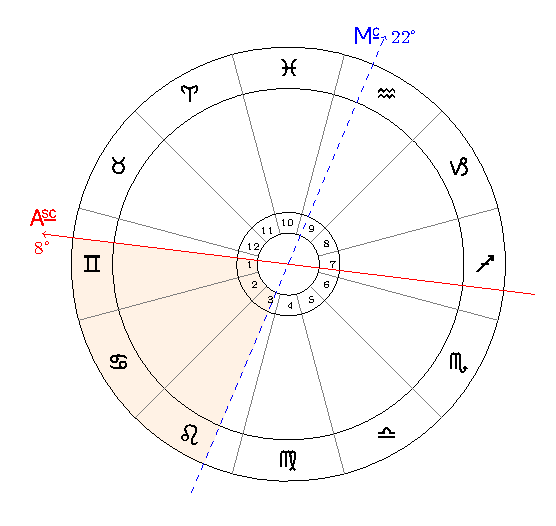
\includegraphics[width=.5\textwidth]{charts/3_03_1}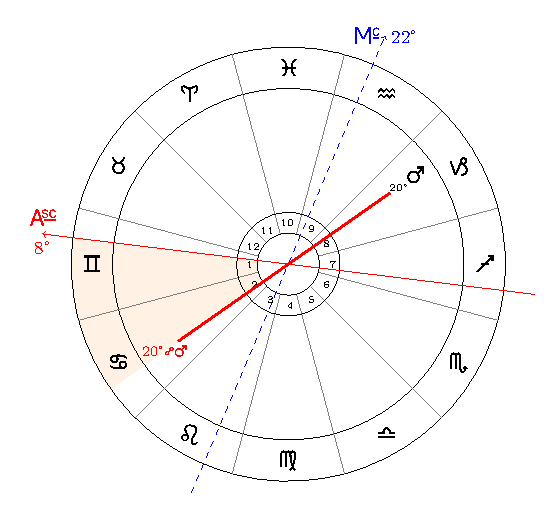
\includegraphics[width=.5\textwidth]{charts/3_03_1a}
\caption{Vital Sector from Asc to IC and ray of malefic}
\end{figure}

If an anaereta is in \Gemini\xspace 20°, or in any degree of \Cancer, or projects its rays to such a point, the native will live as many years as the number of degrees <=rising times> from the aphetic point\footnote{In this example, the aphetic point is the Ascendant.} to the anaeretic point. 

In the same way if we make the vital sector begin at MC, \Aquarius\xspace 22°, we will not find the sum of years to be the distance from MC to the point square with it, \Taurus\xspace 22°, but to \Gemini\xspace 8° <the Ascendant>. 

\begin{figure}[H]
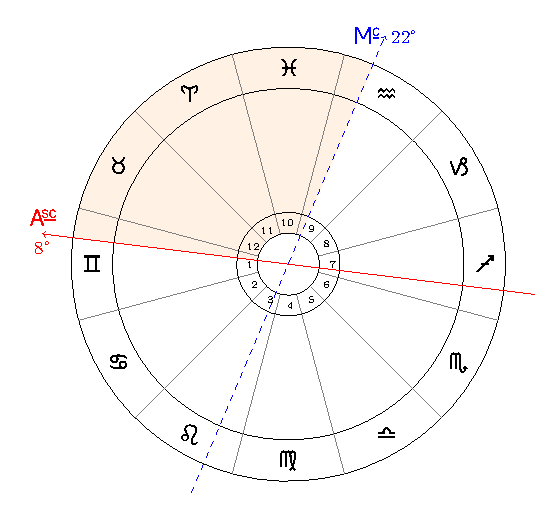
\includegraphics[width=.48\textwidth]{charts/3_03_1b}
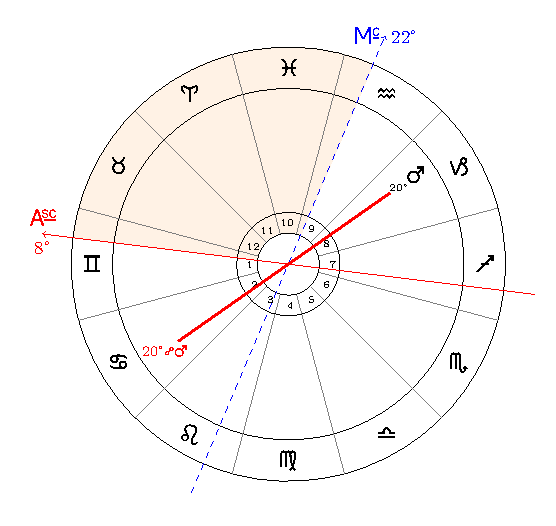
\includegraphics[width=.48\textwidth]{charts/3_03_1c}
\caption{Vital Sector from MC to Asc}
\end{figure}

It is obvious that the vital sector can exceed 90° when using the method of signs, but it cannot exceed the distance to an angle.

Occasionally this latter method can be used with the \Sun\xspace and \Moon, in which case they will exceed 90° if they are helped by houserulers, i.e. when they have houserulers in aspect, favorably situated, and able to allot the full span. In the same example: if we start the vital sector at the Descendant, \Sagittarius\xspace 8°, we will find the end to be at \Aquarius\xspace 22° <MC>. 

In each case, after finding the aphetic place, it will be
necessary to examine the distance to the next angle, and to make the vital sector extend to that position, if no anaereta intercepts.

\index{distribution!primary directions}
Let this further method be regarded as mystically proven in great detail by us: \textbf{/138K/} to treat the degree-position of the apheta as <if it were> MC. With it as MC, it will be necessary to investigate (using the correct klima) which degree can be in the Ascendant. Having found this, make the vital sector extend to that point. 

For example: let the aphetic point be at \Scorpio\xspace 12° in the second klima. If we calculate this as the Ascendant, the vital sector will extend to \Aquarius\xspace 13°, which is IC. But if, as we just stated, we make this point <\Scorpio\xspace 12°> MC, we will find in the table of rising times that \Capricorn\xspace 28° is the Ascendant, and that the vital sector will extend from \Scorpio\xspace 12° to \Capricorn\xspace 28°\footnote{In other words, direct all aphetic points by treating each of them as if they were culminating (at the MC) and determine which degree would be simultaneously rising (at the Asc).}. 

We will find the same to be true for the rest of the nativities or signs. Likewise make the anaeretic position the \textbf{/131P/} Ascendant (as with the aphetic point) and, while it is
the Ascendant, examine which degree of which sign can be MC. Make the vital sector extend to that position or to the point in opposition. In addition calculate in detail the relationships of the houseruler (as we stated above), and examine the distance to the next angle, the configuration of the horoscope, and the combinations of the stars and the apheta.

\begin{figure}[H]
\centering
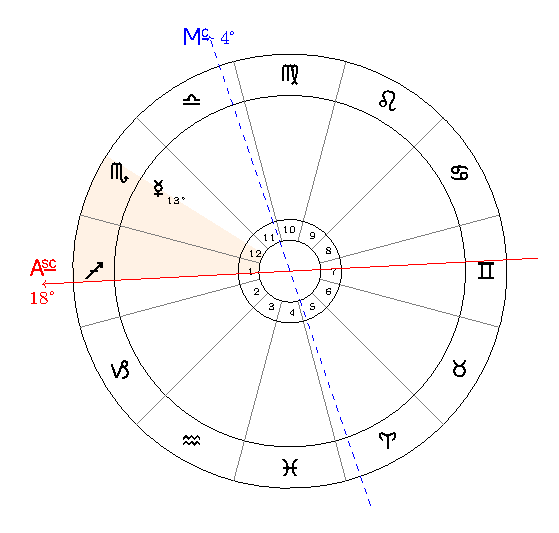
\includegraphics[width=.7\textwidth]{charts/3_03_2}
\caption{Vital Sector from Asc to the apheta}
\end{figure}

An example: let the Ascendant be \Sagittarius\xspace 18°, MC \Libra\xspace 4°, and the houseruler \Mercury\xspace\footnote{The Ascendant (the controller) at 18 \Sagittarius\, falls in the terms (bounds) of \Mercury, making him the houseruler.} at
<\Scorpio> 13°. I calculate the distance from it <\Mercury> to the Ascendant as 35°, which equals 2 1/3 hours\footnote{Fifteen degrees equals one hour (360° / 24 hours), 35° divided by 15° gives 2 1/3 hours.}. Now since 76\footnote{\Mercury's major years are 76.} is assigned as the full span of years, I divide this by 12\footnote{Robert Hand says 12 is used rather than 24 to represent 180° from the Ascendant to Descendant rather than a full 360° (VRS3 p40).} <hours> and find for each hour, 6 years 4 months. So for the 2 hours we find 12 years 8 months, plus (for the one-third hour) 2 years 1 month 10 days. The total is 14 years 9 months 10 days. I subtract this from 76, and the result is 61 years 2 months 20 days. (It is necessary to calculate in the same way if you subtract from the other angles.)

Having established this, now let the \Moon\xspace be the apheta at \Libra\xspace 8°. For the remaining 22° <of \Libra> I assign 29 years 4 months; for the 30° of \Scorpio, 36 years; and for the 17° of \Sagittarius, 18 years 1 month 18 days. Added, the total of the vital sector is 83 years 5 months 18 days
\footnote{He is not calculating the vital sector and the MC of the moon according to \textsl{sphaera recta} (Right Ascension), but by using the rising times of the signs - marginal note [Riley].

Robert Hand shows the calculations using the rising times (oblique ascensions) for each sign: \Libra\, 40°, \Scorpio\, 36°, and \Sagittarius\, 32° (VRS3 p41) so (22/30 x 40°) + 36° + (17/30 x 32°) = 29.33 + 36 + 18.13 = 83.46 $\approx$ 83y 5m 16d. (difference due to rounding fractions)}.

\begin{figure}[H]
\centering
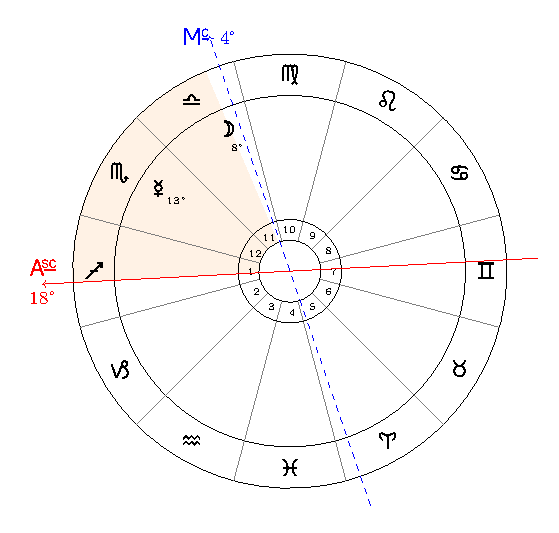
\includegraphics[width=.7\textwidth]{charts/3_03_2a}
\caption{Vital Sector to apheta or controller}
\end{figure}

Now since the years of the apheta are more than the years of the houseruler, the native will live as many years as the
houseruler, \Mercury, allots: 61 years 2 months 20 days. \textbf{/139K/} If the years of the apheta were less than
those of the houseruler and suffered a deduction because of a destructive ray, e.g. at 53 years, it would happen that the cited nativity would live only 53 years. If, however, the houseruler is found to be at an angle and rising, or happens to be in operative degrees\footnote{In the example the operative degrees would be measured from the MC to the Ascendant with the first 1/3 covering 4 \Libra\, to 28 \Libra\, and and the 2nd third running from 28 \Libra\, to 23 \Scorpio, so \Mercury\, is in middling rather than powerful degrees and presumably cannot grant his full 76 years.}, even though the vital sector has more years, the houseruler will allot its total span. 

If the houseruler is favorably located, the destructive stars, even in conjunction or projecting their rays, will no longer shorten the length of life. 

\index{planets!anaeretic}
\index{places!anaeretic}
\index{degrees!anaeretic}
If the nativity is found to lack a houseruler in the vital sector, it will then be necessary to examine the affiliations of the anaeretic stars or their aspects, whether sextile, trine, square, or opposition. The \mn{anaeretic stars} anaeretic stars are \Saturn, \Mars, the \Sun, and the \Moon\xspace coming to a phase\footnote{While about to begin a new phase?}. 

The \mn{anaeretic places} anaeretic places of each sign are the aphetic terms\footnote{The Control is the apheta, which is either a light, the Asc, MC, or syzygy none of which rule terms, so, the ``aphetic terms'' may actually refer to the terms of the Control's term ruler.} and the terms of malefics. 

The \mn{anaeretic degrees} anaeretic degrees are considered to be \textbf{/132P}/ the 3° on each side of the apheta, because each 3° segment either preceding or following has the same effect as conjunction or equivalent degree-position. As a result, the degree itself <of the apheta> plus the two segments total 7° in all. Malefics projecting rays into this area become anaeretic, while benefics prevent the destruction.

For example: let a nativity have \Aries\xspace 12° as the Ascendant. This point will be the midpoint <of the segment \Aries\xspace 9°> to \Aries\xspace 15°. If a malefic projects rays into the arc from \Aries\xspace 9° to \Aries\xspace 15°, it will be destructive in these degrees, not only in the sign of the vital sector, but in the other signs from the apheta
to the point square with it. 

For example: if \Aries\xspace is the Ascendant, and if \Saturn\xspace or \Mars\xspace are found at \Taurus\xspace 15° or \Gemini\xspace 15°, and if the vital sector comes to \Taurus\xspace 12° or 13° or to \Gemini\xspace 12° or 13° in
the sequence of chronocratorships, there will be destructive action.

\index{planets!destructive}
If the destructive stars are at or just following an angle, they become more active; if they are not at an angle, they are weakened. Let this method be most effective for those at an angle. 

For example: \Aries\xspace is the Ascendant as cited above, and \Saturn\xspace is at \Sagittarius\xspace 13°, 12° or even 20°. Figured by signs, it just precedes MC, but since it projects its rays into an angle and into operative places (viz. into \Aries, which is \Trine\xspace <with \Sagittarius>), it will be considered the anaereta. If, however, \Saturn\xspace is found in \Sagittarius\xspace 3° or 7°, it will precede an angle both by degrees and according to signs, and it will not be the anaereta. This happens \textbf{/140K/} because an anaereta which projects rays from an angle into inoperative degrees which precede an angle does not become destructive. All this also applies to benefics.

\begin{figure}[H]
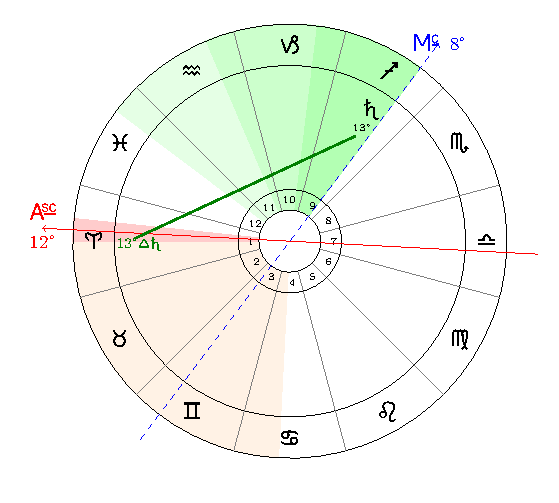
\includegraphics[width=.48\textwidth]{charts/3_03_3a}
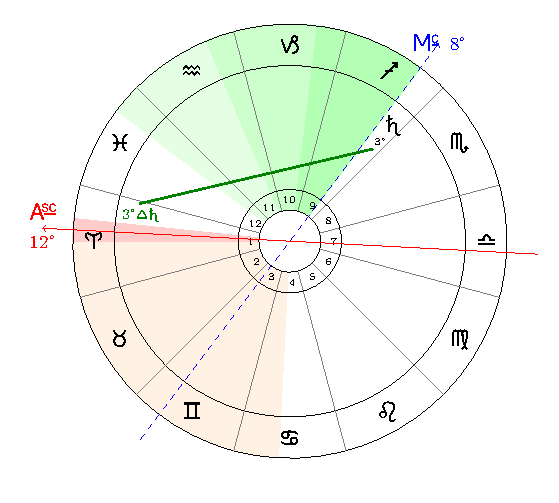
\includegraphics[width=.48\textwidth]{charts/3_03_3b}
\caption{Destructive and non-Destructive Rays}
\end{figure}
\newpage
\begin{mdframed}[backgroundcolor=cyan!5]
\textbf{Comment:}

The charts show an example of \Saturn\, sending destructive and non-destructive trines to the 7° range of degrees around the Ascendant. The peach shading represents the vital sector; the green, operative degrees from the MC to the Ascendant.

In the chart on the left, \Saturn\, is in operative degrees, in the chart on the right, he is not. It does not seem to matter, in either case, whether or not the other end of the aspect falls on operative degrees but only that it falls with the 7° range of the aphetic point being aspected.
\end{mdframed}

\newpage
